%!TeX root = paper22-coord-ac-rl.tex
\begin{figure}[t]
  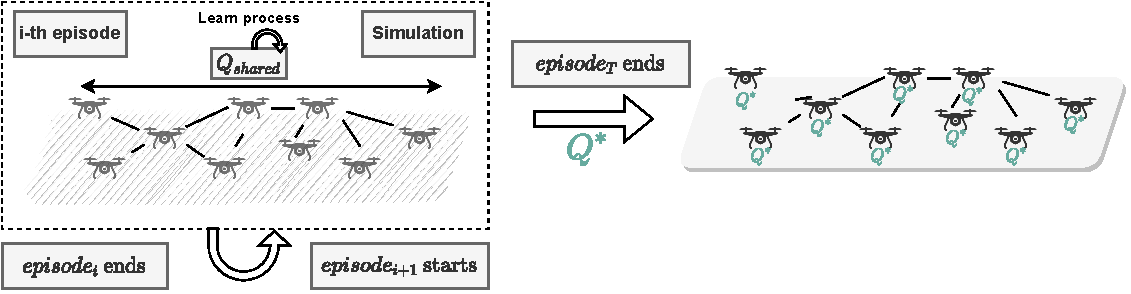
\includegraphics[width=\textwidth]{papers/coordination2022/img/algorithm-learning.pdf}
  \caption[Reinforcement Learning schema used in program synthesis simulations]{
  Reinforcement Learning schema used in our simulations.
  The learning algorithm is applied at simulation time (for $T$ episodes) improving a shared $Q$ table. 
  %
  At the deployment time then, the agents exploit a local copy of the optimal $Q^*$ table found by learning.}
  \label{coordination2022:fig:learning-scheme}
\end{figure}